% Layout für Felix' Sachkunde-Lernmaterial (LuaLaTeX).
% Wird über _metadata.yml in alle Blätter dieses Ordners eingebunden.
% Angelehnt an unterricht/mathematik/klasse-05/arithmetik/foerdermaterial-online/foerder-header.tex,
% aber für Grundschule: größere Schrift, mehr Luft, keine Mathe-Zeichnungen.
% Überschriften: CutePixel (Systemschrift), Fließtext: TeX Gyre Heros.

\usepackage{unicode-math}
\setmathfont{TeX Gyre Pagella Math}
\usepackage[nobottomtitles*]{titlesec}
\renewcommand{\bottomtitlespace}{0.14\textheight}
\usepackage{colortbl}
\usetikzlibrary{patterns,shapes.geometric,shapes.callouts,decorations.pathreplacing,arrows.meta,positioning,fit,backgrounds,calc}
\tcbuselibrary{skins,breakable}

\setmainfont{TeX Gyre Heros}[Scale=1.0]
\setsansfont{TeX Gyre Heros}[Scale=1.0]
\newfontfamily\pixelfont{CutePixel}[Scale=1]
\renewcommand{\headingfont}{\pixelfont}

% ---------- Farben ----------
\definecolor{pxink}{HTML}{1E1B3A}
\definecolor{pxblue}{HTML}{2F5BEA}
\definecolor{pxbluelight}{HTML}{E3EBFF}
\definecolor{pxgreen}{HTML}{15966A}
\definecolor{pxgreenlight}{HTML}{DDF4E9}
\definecolor{pxorange}{HTML}{F08A24}
\definecolor{pxorangelight}{HTML}{FFEBD2}
\definecolor{pxred}{HTML}{DB3A56}
\definecolor{pxredlight}{HTML}{FFE1E6}
\definecolor{pxyellow}{HTML}{FFC933}
\definecolor{pxyellowlight}{HTML}{FFF6D6}
\definecolor{pxpurple}{HTML}{7A4FD1}
\definecolor{pxpurplelight}{HTML}{EDE5FA}
\definecolor{pxgray}{HTML}{8E8CA3}
\colorlet{examprimary}{pxblue}
\colorlet{examprimarylight}{pxbluelight}
\colorlet{examink}{pxink}
\definecolor{examlightgray}{HTML}{FBF8EC}
\colorlet{exammidgray}{pxgray}
\colorlet{examrulegray}{pxgray!70}
\AtBeginDocument{\color{pxink}}

% ---------- Überschriften ----------
\newcommand{\pxbadge}[1]{%
  \tikz[baseline=(pxb.base)]{%
    \node[inner xsep=2.2mm,inner ysep=1.1mm,fill=pxyellow,draw=pxink,line width=0.8pt,font=\pixelfont\fontsize{12}{13}\selectfont,text=pxink] (pxb) {#1};
    \begin{scope}[on background layer]
      \fill[pxink] ([shift={(0.7mm,-0.7mm)}]pxb.south west) rectangle ([shift={(0.7mm,-0.7mm)}]pxb.north east);
    \end{scope}}}
\titleformat{\section}[block]{}{}{0pt}{\pxbadge}
\titleformat{\subsection}[block]{}{}{0pt}{\pxbadge}
\titlespacing*{\section}{0pt}{1.2ex plus 0.3ex}{1.0ex}
\titlespacing*{\subsection}{0pt}{1.2ex plus 0.3ex}{1.0ex}

% ---------- Blattkopf ----------
% \blattkopf{Titel}{Untertitel}  -- Untertitel darf leer sein.
% Name/Datum nur auf geraden Seiten (Rückseite), wie im Fördermaterial.
\newcommand{\blattkopf}[2]{%
  \begin{center}
  \lefthyphenmin=99 \righthyphenmin=99 \hyphenpenalty=10000 \exhyphenpenalty=10000
  {\pixelfont\fontsize{21}{24}\selectfont\color{pxink}\begin{minipage}{0.96\linewidth}\centering #1\end{minipage}\par}
  \ifstrempty{#2}{}{\vspace{1.2mm}{\small\color{pxgray}#2\par}}
  \end{center}
  \vspace{0.6mm}
}
\newcommand{\namenszeile}{%
  \noindent\begin{tabularx}{\linewidth}{@{}Xr@{}}
  Name: \fieldline[6.4cm] & Datum: \fieldline[3cm]
  \end{tabularx}\par\vspace{2mm}}

% ---------- Aufgabennummern ----------
\newlength{\pxnumw}
\newcommand{\tasknum}[1]{%
  \par\needspace{2.6\baselineskip}\begingroup\setlength{\fboxsep}{1.8pt}\pixelfont\fontsize{11}{11}\selectfont
  \settowidth{\pxnumw}{#1}\ifdim\pxnumw<3mm\setlength{\pxnumw}{3mm}\fi
  \raisebox{-0.5pt}{\colorbox{pxink}{\makebox[\pxnumw]{\color{white}#1}}}%
  \endgroup\hspace{1.4mm}}

% ---------- Schreibfelder ----------
\newcommand{\blank}[1][3cm]{\mbox{\rule{0pt}{0.5cm}\textcolor{pxgray}{\rule{#1}{0.6pt}}}}
\newcommand{\platz}[1][1.5cm]{\raisebox{-1mm}{\tcbox[on line,enhanced,colback=pxyellowlight,colframe=pxyellowlight,sharp corners,boxrule=0pt,borderline={0.6pt}{0pt}{pxink!70,dashed},boxsep=0pt,left=0.5mm,right=0.5mm,top=0.3mm,bottom=0.3mm,height=0.55cm,valign=center]{\makebox[#1]{}}}}
% Linien zum Schreiben: \linien{Anzahl}
\newcommand{\linien}[1]{\par\vspace{1mm}\begingroup\setlength{\parskip}{0pt}%
  \foreach \n in {1,...,#1}{\noindent\textcolor{pxgray}{\rule{\linewidth}{0.6pt}}\par\vspace{7.5mm}}%
  \endgroup\vspace{-6mm}\par}
% Kariertes/leeres Schreibfeld mit gestricheltem Rand: \workbox{Höhe}
\newcommand{\workbox}[1]{\par\vspace{0.6mm}\noindent\begin{tikzpicture}
  \pgfmathtruncatemacro{\pxrows}{floor(#1/0.75cm)}
  \fill[white] (0,0) rectangle (\linewidth,#1);
  \foreach \r in {1,...,\pxrows}{%
    \draw[pxgray!55,line width=1.1pt,line cap=round,dash pattern=on 0pt off 5mm] (2.5mm,{\r*0.75cm-0.375cm}) -- ({\linewidth-1mm},{\r*0.75cm-0.375cm});}
  \draw[pxink!70,dashed,line width=0.6pt] (0,0) rectangle (\linewidth,#1);
\end{tikzpicture}\par}

% ---------- Kästen ----------
% #1 Titel, #2 kräftige Farbe, #3 helle Farbe, #4 Inhalt
\newcommand{\pxbox}[4]{%
  \par\vspace{1.4mm}
  \begin{tcolorbox}[enhanced,breakable,sharp corners,colback=#3,colframe=#2,boxrule=0.9pt,
    left=2.2mm,right=2.2mm,top=2.2mm,bottom=1.0mm,before skip=0pt,after skip=1.8mm,
    shadow={0.9mm}{-0.9mm}{0mm}{fill=pxink,opacity=1},
    attach boxed title to top left={xshift=3mm,yshift=-2.2mm},
    boxed title style={sharp corners,colback=#2,colframe=#2,boxrule=0pt,top=0.5mm,bottom=0.3mm,left=1.3mm,right=1.3mm},
    fonttitle=\pixelfont\normalsize\color{white},title={#1}]#4\end{tcolorbox}\par}
\newcommand{\lernbox}[1]{\pxbox{Darum geht es}{pxblue}{pxbluelight}{#1}}
\newcommand{\denkbox}[1]{\pxbox{Merke}{pxorange}{pxorangelight}{#1}}
\newcommand{\wissenbox}[1]{\pxbox{Das steht im Heft}{pxgreen}{pxgreenlight}{#1}}
\newcommand{\hinweisbox}[1]{\pxbox{Tipp}{pxgray}{white}{#1}}
\newcommand{\elternbox}[1]{\pxbox{Für Mama oder Papa}{pxgray}{white}{\footnotesize #1}}
% Der Strategie-Kasten macht sichtbar, WELCHE Lernstrategie das Blatt gerade übt.
% #1 Name der Strategie, #2 Erklärung in einem Satz.
\newcommand{\strategie}[2]{%
  \par\vspace{1.2mm}
  \begin{tcolorbox}[enhanced,sharp corners,colback=pxpurplelight,colframe=pxpurple,boxrule=0.9pt,
    left=2.2mm,right=2.2mm,top=2.2mm,bottom=1.0mm,before skip=0pt,after skip=1.8mm,
    shadow={0.9mm}{-0.9mm}{0mm}{fill=pxink,opacity=1},
    attach boxed title to top left={xshift=3mm,yshift=-2.2mm},
    boxed title style={sharp corners,colback=pxpurple,colframe=pxpurple,boxrule=0pt,top=0.5mm,bottom=0.3mm,left=1.3mm,right=1.3mm},
    fonttitle=\pixelfont\normalsize\color{white},title={Lernstrategie}]%
    \textbf{#1}\par\vspace{0.8mm}#2\end{tcolorbox}\par}
% Selbstkontrolle: #1 Aufgabe, #2 Lösungen
\newcommand{\selbstcheck}[2]{%
  \par\vspace{1.2mm}
  \begin{tcolorbox}[enhanced,breakable,sharp corners,colback=pxbluelight,colframe=pxblue,boxrule=0.9pt,
    left=2.2mm,right=2.2mm,top=2.2mm,bottom=1.0mm,before skip=0pt,after skip=1.8mm,
    shadow={0.9mm}{-0.9mm}{0mm}{fill=pxink,opacity=1},
    attach boxed title to top left={xshift=3mm,yshift=-2.2mm},
    boxed title style={sharp corners,colback=pxblue,colframe=pxblue,boxrule=0pt,top=0.5mm,bottom=0.3mm,left=1.3mm,right=1.3mm},
    fonttitle=\pixelfont\normalsize\color{white},title={Teste dich selbst!}]%
    #1\par\vspace{-0.6mm}\noindent\textcolor{pxblue}{\dotfill}\par\vspace{0.6mm}%
    {\footnotesize\textbf{Lösungen:} #2}\end{tcolorbox}\par}
% Lösungsblock am Blattende, damit Felix ohne Erwachsenen kontrollieren kann.
\newcommand{\loesungen}[1]{%
  \par\vspace{1.4mm}
  \begin{tcolorbox}[enhanced,breakable,sharp corners,colback=white,colframe=pxgray,boxrule=0.9pt,
    left=2.2mm,right=2.2mm,top=2.2mm,bottom=1.0mm,before skip=0pt,after skip=1.4mm,
    attach boxed title to top left={xshift=3mm,yshift=-2.2mm},
    boxed title style={sharp corners,colback=pxgray,colframe=pxgray,boxrule=0pt,top=0.5mm,bottom=0.3mm,left=1.3mm,right=1.3mm},
    fonttitle=\pixelfont\normalsize\color{white},title={Lösungen zum Selberkontrollieren}]%
    \footnotesize #1\end{tcolorbox}\par}

% ---------- Zwei Spalten mit Trennstrich ----------
\newcommand{\zweispalten}[2]{\par\noindent{\setlength{\tabcolsep}{0pt}\begin{tabular}{@{}p{0.465\linewidth}@{\hspace{3mm}}!{\color{pxgray}\vrule width 0.7pt}@{\hspace{3mm}}p{0.465\linewidth}@{}}#1&#2\end{tabular}}\par}
\newcommand{\zweispaltenoffen}[2]{\par\noindent{\setlength{\tabcolsep}{0pt}\begin{tabular}{@{}p{0.48\linewidth}@{\hspace{4mm}}p{0.48\linewidth}@{}}#1&#2\end{tabular}}\par}

% ---------- Tabellen ----------
\arrayrulecolor{pxink}
\setlength{\arrayrulewidth}{0.6pt}
\newcommand{\kopf}{\rowcolor{pxbluelight}}

% ---------- Kette aus Kästchen mit Pfeilen (Atemweg, Verdauungsweg) ----------
% \kette{Text1,Text2,...}  -- bricht automatisch um, "?" ergibt ein leeres Feld
\newcommand{\kettenglied}[1]{%
  \tikz[baseline=(kg.base)]{\node[draw=pxink,line width=0.8pt,fill=pxbluelight,sharp corners,
    inner xsep=1.8mm,inner ysep=1.3mm,font=\small,text=pxink,minimum width=1.6cm,align=center] (kg) {#1};}}
\newcommand{\kettenleer}[1][2.4cm]{%
  \tikz[baseline=(kg.base)]{\node[draw=pxink,line width=0.8pt,dashed,fill=pxyellowlight,sharp corners,
    inner xsep=1.8mm,inner ysep=1.3mm,font=\small,text=pxink,minimum width=#1,align=center] (kg) {\vphantom{Ag}};}}
\newcommand{\kpfeil}{\;\textcolor{pxink}{\raisebox{0.3ex}{\scriptsize$\blacktriangleright$}}\;}

% ---------- Blutkreislauf-Schema ----------
% Lunge oben, Herz in der Mitte, Koerper unten. Links laeuft das sauerstoffarme
% Blut (blau), rechts das sauerstoffreiche (rot). Innerer Korridor = kleiner
% Kreislauf, aeusserer Korridor = grosser Kreislauf.
% #1 Beschriftung Lunge, #2 Herz, #3 Koerper (leer lassen fuer das Ausfuellblatt)
\newcommand{\kreislaufschema}[3]{%
\begin{center}
\begin{tikzpicture}[x=1cm,y=1cm,font=\small,
  ader/.style={line width=1.5pt,-{Stealth[length=3mm,width=2.4mm]},rounded corners=2mm}]
  \node[draw=pxink,line width=0.9pt,fill=pxbluelight,sharp corners,
        minimum width=3.4cm,minimum height=1.1cm,align=center] (lunge)   at (0,3.3) {#1};
  \node[draw=pxink,line width=0.9pt,fill=pxredlight,sharp corners,
        minimum width=3.4cm,minimum height=1.1cm,align=center] (herz)    at (0,1.4) {#2};
  \node[draw=pxink,line width=0.9pt,fill=pxbluelight,sharp corners,
        minimum width=3.4cm,minimum height=1.1cm,align=center] (koerper) at (0,-0.5) {#3};
  % kleiner Kreislauf: Herz -> Lunge (blau, innen links), Lunge -> Herz (rot, innen rechts)
  \draw[ader,pxblue] (-1.7,1.65) -- (-2.7,1.65) -- (-2.7,3.55) -- (-1.7,3.55);
  \draw[ader,pxred]  ( 1.7,3.05) -- ( 2.7,3.05) -- ( 2.7,1.15) -- ( 1.7,1.15);
  % grosser Kreislauf: Herz -> Koerper (rot, aussen rechts), Koerper -> Herz (blau, aussen links)
  \draw[ader,pxred]  ( 1.7,1.65) -- ( 4.2,1.65) -- ( 4.2,-0.25) -- ( 1.7,-0.25);
  \draw[ader,pxblue] (-1.7,-0.75) -- (-4.2,-0.75) -- (-4.2,1.15) -- (-1.7,1.15);
  \node[font=\footnotesize\bfseries,text=pxink,align=center] at (-4.4,3.3) {kleiner\\Kreislauf};
  \node[font=\footnotesize\bfseries,text=pxink,align=center] at ( 5.9,-0.5) {gro\ss{}er\\Kreislauf};
\end{tikzpicture}
\par\vspace{1.5mm}{\footnotesize\textcolor{pxblue}{\rule{7mm}{1.5pt}} sauerstoffarmes Blut \qquad \textcolor{pxred}{\rule{7mm}{1.5pt}} sauerstoffreiches Blut}
\end{center}}

% ---------- Beuger und Strecker ----------
% Schematischer Arm mit Pfeilen auf die beiden Muskellagen am Oberarm.
% \armbild{gebeugt} oder \armbild{gestreckt}
\newcommand{\armbild}[1]{%
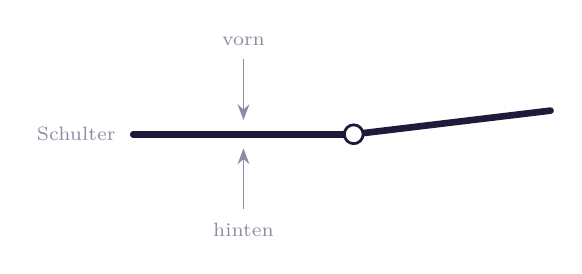
\begin{tikzpicture}[x=1cm,y=1cm,font=\footnotesize]
  % Oberarm waagerecht, Schulter links, Ellenbogen bei (2.8,0)
  \draw[pxink,line width=2.4pt,line cap=round] (0,0) -- (2.8,0);
  \ifstrequal{#1}{gebeugt}%
    {\draw[pxink,line width=2.4pt,line cap=round] (2.8,0) -- (3.8,2.1);}%
    {\draw[pxink,line width=2.4pt,line cap=round] (2.8,0) -- (5.3,0.3);}%
  \fill[white] (2.8,0) circle (3.4pt);
  \draw[pxink,line width=1pt] (2.8,0) circle (3.4pt);
  \node[font=\scriptsize,text=pxgray,left=1mm] at (0,0) {Schulter};
  % Zeiger auf Vorder- und Rueckseite des Oberarms
  \draw[pxgray,line width=0.7pt,-{Stealth[length=2mm]}] (1.4,0.95) -- (1.4,0.18);
  \draw[pxgray,line width=0.7pt,-{Stealth[length=2mm]}] (1.4,-0.95) -- (1.4,-0.18);
  \node[font=\scriptsize,text=pxgray,above] at (1.4,1.0) {vorn};
  \node[font=\scriptsize,text=pxgray,below] at (1.4,-1.0) {hinten};
\end{tikzpicture}}

% ---------- Lernkarten ----------
% Ein Kartenblatt trägt 2 Spalten x 4 Zeilen. Kartengröße 8.4cm x 5.9cm.
\newlength{\kartebreite}\setlength{\kartebreite}{8.4cm}
\newlength{\kartehoehe}\setlength{\kartehoehe}{6.3cm}
\newlength{\karterand}\setlength{\karterand}{3.2mm}
% Grundgerüst einer Karte: #1 Hintergrundfarbe, #2 Inhalt. Inhalt steht oben.
\newcommand{\kartenrahmen}[2]{%
  \begin{tikzpicture}
    \node[draw=pxink,line width=0.7pt,dashed,fill=#1,sharp corners,inner sep=\karterand,
          anchor=south west] at (0,0)
    {\begin{minipage}[t][\dimexpr\kartehoehe-2\karterand\relax][t]{\dimexpr\kartebreite-2\karterand\relax}%
       \setlength{\parskip}{0pt}\setlength{\parindent}{0pt}\raggedright #2%
     \end{minipage}};
  \end{tikzpicture}}
% Vorderseite: #1 Thema (kleines Etikett), #2 Frage
\newcommand{\kartev}[2]{\kartenrahmen{white}{%
  {\pixelfont\fontsize{8}{9}\selectfont\textcolor{pxgray}{#1}}\par\vspace{2.5mm}
  {\normalsize\textbf{#2}}}}
% Rückseite: #1 Antwort
\newcommand{\karter}[1]{\kartenrahmen{pxyellowlight}{\small #1}}
% Rückseite zum Selberschreiben: Linien
\newcommand{\karterleer}{\kartenrahmen{white}{%
  {\pixelfont\fontsize{8}{9}\selectfont\textcolor{pxgray}{Antwort}}\par\vspace{1mm}
  \textcolor{pxgray}{\rule{\linewidth}{0.5pt}}\par\vspace{5.5mm}
  \textcolor{pxgray}{\rule{\linewidth}{0.5pt}}\par\vspace{5.5mm}
  \textcolor{pxgray}{\rule{\linewidth}{0.5pt}}\par\vspace{5.5mm}
  \textcolor{pxgray}{\rule{\linewidth}{0.5pt}}\par\vspace{5.5mm}
  \textcolor{pxgray}{\rule{\linewidth}{0.5pt}}}}
% Ganz leere Karte zum Selbermachen
\newcommand{\karteblanko}[1]{\kartenrahmen{white}{%
  {\pixelfont\fontsize{8}{9}\selectfont\textcolor{pxgray}{#1}}\par\vspace{1mm}
  \textcolor{pxgray}{\rule{\linewidth}{0.5pt}}\par\vspace{5.5mm}
  \textcolor{pxgray}{\rule{\linewidth}{0.5pt}}\par\vspace{5.5mm}
  \textcolor{pxgray}{\rule{\linewidth}{0.5pt}}\par\vspace{5.5mm}
  \textcolor{pxgray}{\rule{\linewidth}{0.5pt}}\par\vspace{5.5mm}
  \textcolor{pxgray}{\rule{\linewidth}{0.5pt}}}}
% Eine Zeile mit zwei Karten
\newcommand{\kartenzeile}[2]{\noindent#1\hfill#2\par\vspace{0mm}}

% ---------- Ausfülltabelle, linksbündig über die volle Breite ----------
% Zeilen: Text & \platz[5cm]\\[1.5mm]
\newcommand{\fuelltabelle}[2]{\par\vspace{1mm}\noindent\begin{tabularx}{\linewidth}{@{}X@{}p{#1}@{}}#2\end{tabularx}\par\vspace{1mm}}
% Kästchen zum Ankreuzen
\newcommand{\kreuz}{$\square$}

% ---------- Kartenblatt ----------
% Eine Seite trägt 2 Spalten x 4 Zeilen. Innerhalb der Umgebung sind Absatz-
% abstände abgeschaltet, damit die Karten bündig aneinander liegen.
\newenvironment{kartenblatt}{%
  \thispagestyle{empty}\par\begingroup
  \setlength{\parskip}{0pt}\setlength{\parindent}{0pt}\setlength{\lineskip}{0pt}%
  \setlength{\baselineskip}{0pt}\par\nointerlineskip}{\par\endgroup}
% Eine Zeile mit zwei Karten
\renewcommand{\kartenzeile}[2]{\noindent#1\hfill#2\par\vspace{1.5mm}}
% Karte einmal definieren, vorne und hinten getrennt abrufen.
% \karte{Kürzel}{Thema}{Frage}{Antwort}   dann \kv{Kürzel} bzw. \kr{Kürzel}
\makeatletter
\newcommand{\karte}[4]{%
  \expandafter\gdef\csname sk@v@#1\endcsname{\kartev{#2}{#3}}%
  \expandafter\gdef\csname sk@r@#1\endcsname{\karter{#4}}}
\newcommand{\kv}[1]{\csname sk@v@#1\endcsname}
\newcommand{\kr}[1]{\csname sk@r@#1\endcsname}
\makeatother

% Namenszeile im Seitenkopf abschalten (Heimmaterial braucht sie nicht).
\newcommand{\ohnenamen}{\examshownameheaderfalse}
